\documentclass[10pt,a4paper,twoside,twocolumn]{article}%ustalasz jaki typ dokumentu i właściwości

\usepackage[polish]{babel} % ustawianie języka polskiego
\usepackage[colorlinks=false,linkcolor=green,urlcolor=green,citecolor=green]{hyperref}%hiperłącza ogólnego rodzaju
\hypersetup{pdftitle=Sprawozdanie SSR}

\usepackage{pdfpages} % importowanie plików z pdfa
\usepackage{amsmath} % do wstawiania macierz itp
\usepackage{graphicx} % wstawianie zdjęć
% \usepackage[utf8]{inputenc} % niepotrzebne bo lualatex
\usepackage[T1]{fontenc} % niepotrzebne bo lualatex
\usepackage[left=1cm,right=1cm,top=1cm,bottom=2cm,
columnsep=1cm % odstęp między kolumnami
]{geometry}%marginesy

\usepackage{listings} % punktowanie
% \usepackage{indentfirst} % dawanie akapitu na początku
\usepackage{caption} % podpisy
\usepackage{subcaption} % podpisy do subfigure
\usepackage{siunitx} % jednostki si
\usepackage{minted} % ładne kody naprzyklad matlaba
\setminted{linenos=true,frame=single,breaklines=true,breaksymbolleft=,style=vs}

\usepackage{textcase}

\usepackage[polish,nameinlink]{cleveref} % dobre prefiksy przed etykietą i język
\usepackage{cprotect}

\usepackage{fontspec}
% \setmainfont[Ligatures=TeX]{Georgia}
% \setsansfont[Ligatures=TeX]{Arial}
\usepackage{parskip} % usunięcie tab na początku akapitu
\usepackage{newfloat} % aby można było ładnie wstawić elementy typu zdjecie, kod itp

%%% rysowanie wykresów %%% ale w ciul to trudne więc app.diagrams.net
\usepackage{tikz}
\usetikzlibrary{shapes.geometric, arrows, positioning}

% % % SVG import
\usepackage{svg}
\usepackage{import}
\usepackage{xifthen}
\usepackage{transparent}

% \usepackage{mdframed} % ramki
\usepackage[framemethod=TikZ]{mdframed}
\mdfsetup{%
middlelinecolor=red,
middlelinewidth=1pt,
   backgroundcolor=gray!20,
   roundcorner=10pt}

\usepackage{enumitem} % podpunkty customowe

\usepackage{pgfplots}[compat=1.18] % wykresy


%%%%%%%%%%%%%% koniec pakietów %%%%%%%%%%%%%%%%%%%%%%%%%%%

\boldmath%pogrubiona matma

\title{Fajny ten tytuł}%tytuł
\date{\today}%%data
\author{Janusz Chmaruk}%autor
\setcounter{secnumdepth}{3}%głębokość liczenia roździałów

% PRZYKŁAD LICZNIKA ZADAŃ
\newcounter{zadanie}
\newenvironment{zadanie}[1][]{
   \refstepcounter{zadanie}
   \subsection*{Zadanie \thezadanie#1}
   \addcontentsline{toc}{subsection}{Zadanie \thezadanie#1} % dodanie do spisu treści
}{}

% PRZYKŁAD LICZNIKA ROZWIĄZAŃ
\newcounter{rozwiazanie}
\newenvironment{rozwiazanie}[1][]{
   \refstepcounter{rozwiazanie}
   \subsection*{Rozwiazanie zadania \therozwiazanie#1}
   \addcontentsline{toc}{subsection}{Rozwiazanie zadania \therozwiazanie#1} % dodanie do spisu treści
}{}


% DŁUGIE LISTINGI
\newenvironment{longlisting}{\captionsetup{type=listing}}{}

%%%%%%%%%%%%%%%%%%%%%%%%%%%%%%%%%%%%%%%%%%%%%%%%%%%%%%%%%%%%%%%
%%%%%%%%%%%%%%%%%%%%%%%%%%%%%%%%%%%%%%%%%%%%%%%%%%%%%%%%%%%%%%%
%%%%%%% TU SIE ZACZYNA PISANIE PLIKU %%%%%%%%%%%%%%%%%%%%%%%%%%
%%%%%%%%%%%%%%%%%%%%%%%%%%%%%%%%%%%%%%%%%%%%%%%%%%%%%%%%%%%%%%%
%%%%%%%%%%%%%%%%%%%%%%%%%%%%%%%%%%%%%%%%%%%%%%%%%%%%%%%%%%%%%%%

\begin{document}%zaczyna się dokument

\null%
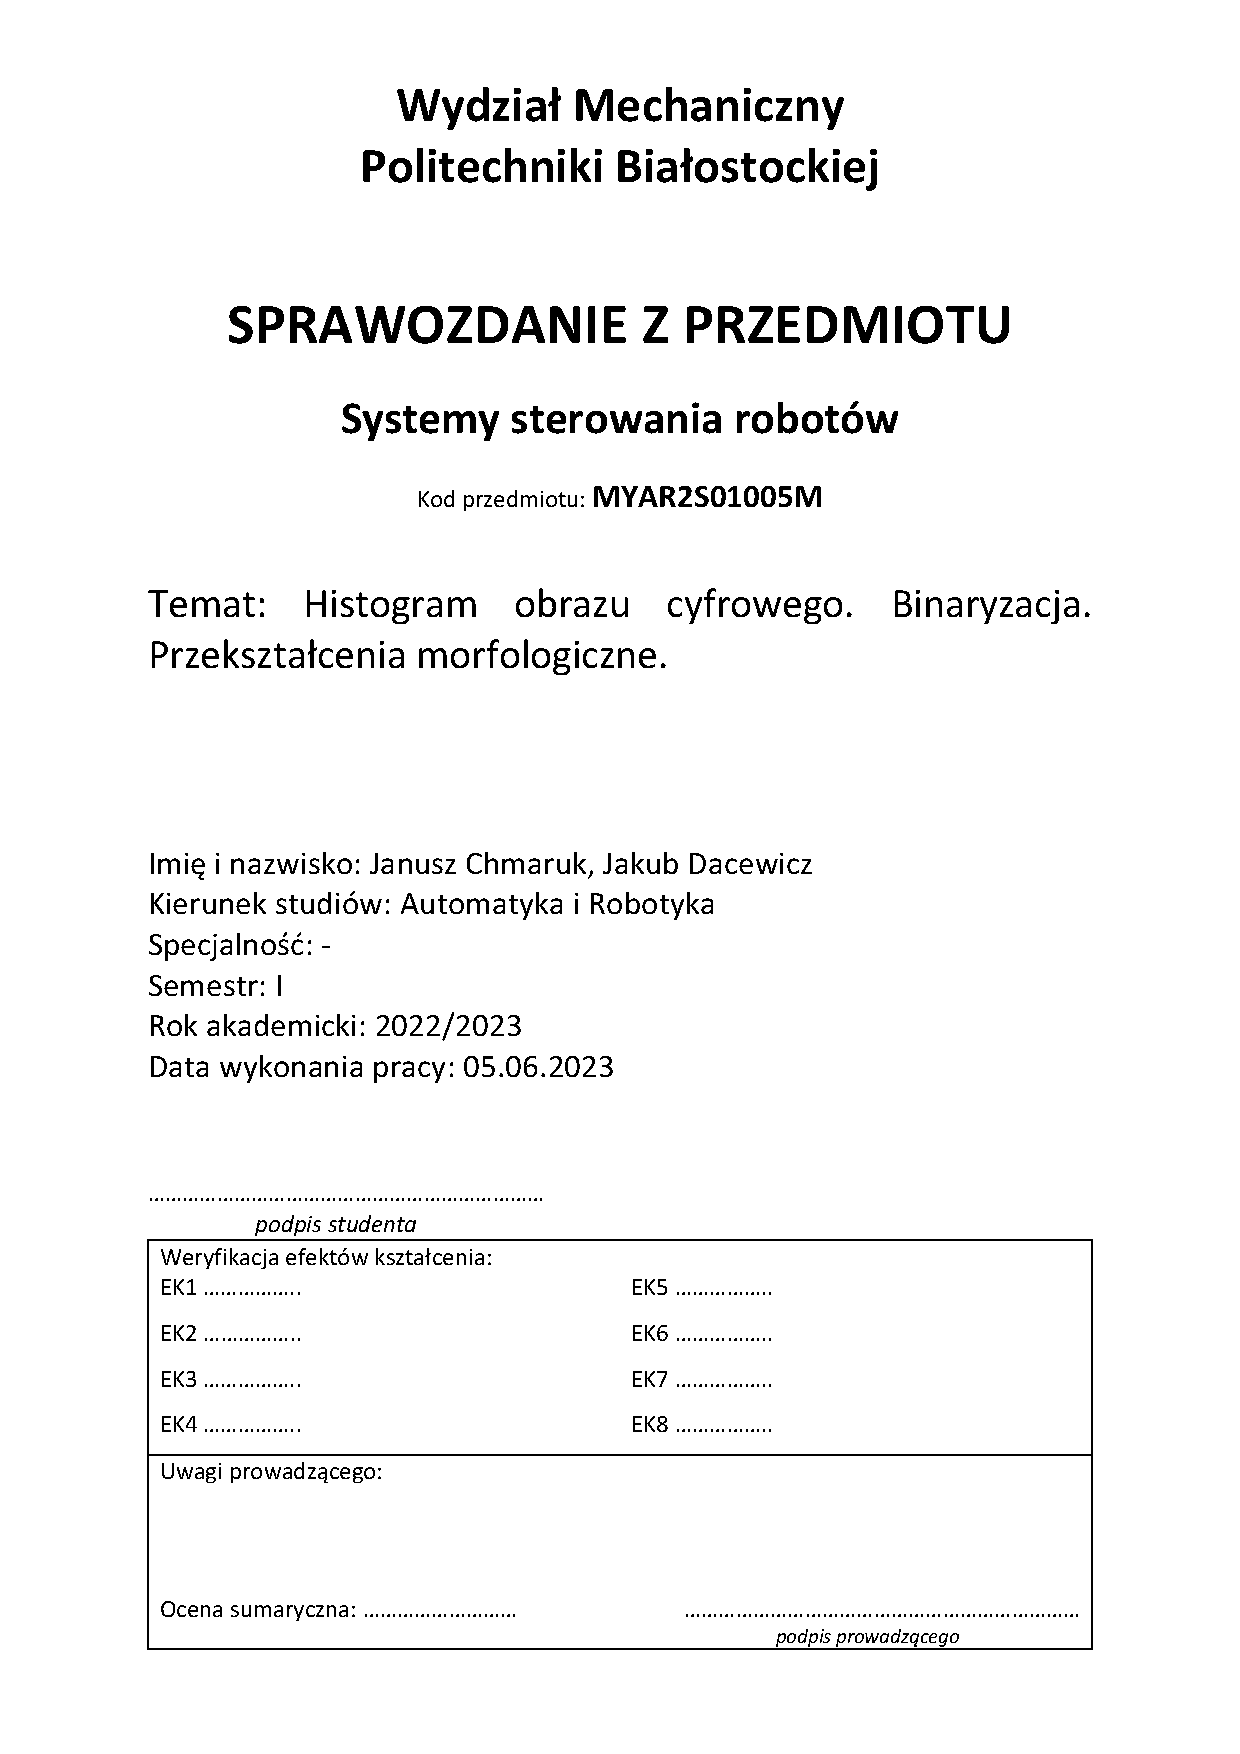
\includepdf[pages={1}]{Szablon_Projektu.pdf}
\clearpage%następna strona ogółem

\tableofcontents%spis treści
% \clearpage

\section{Cel ćwiczenia}
Celem ćwiczenia jest zapoznanie studentów z serwerem parametrów w systemie ROS.

\section{Przebieg ćwiczenia}
W ramach ćwiczenia zapoznamy się z:
\begin{itemize}
    \item definiowaniem parametrów,
    \item obsługą parametrów w językach Python i C++.
\end{itemize}

\section{Zadania do realizacji}
%numeracja z liczbami

\begin{zadanie}[: Modyfikacja przykładowego programu]
    Sprawdź, jak działają umieszczone powyżej programy. Zmodyfikuj program tak, aby reagował na zmianę wartości parametrów w trakcie działania programu.
\end{zadanie}

\begin{zadanie}[: Regulator PID]

    Napisz program implementujący regulator PID\@. Użyj parametrów systemu
    ROS do modyfikacji wartości współczynników kp, ki i kd, a także progów
    saturacji regulatora. Regulator PID (Proportional - Integral -
    Derivative) jest klasycznym regulatorem stosowanym w wielu zastosowaniach
    przemysłowych. Odpowiedź tego regulatora wyznaczana jest na podstawie
    sygnału błędu, całki tego sygnału, oraz jego pochodnej (najczęściej
    wyznaczanej metodami numerycznymi). Jedną z prostych możliwych realizacji
    algorytmu regulatora PID można przedstawić przy pomocy poniższego pseudokodu:
    \begin{verbatim}
e := y_zadane - y_mierzone
e_i := e_i + e * dt
e_d := (e - e_poprzednie) / dt
e_poprzednie := e
u := kp * e + ki * e_i + kd * e_d
    \end{verbatim}
    W powyższym pseudokodzie, y\_zadane oznacza wartość zadaną sygnału
    regulowanego, a y mierzone jego aktualną wartość mierzoną. Sygnał e oznacza
    aktualną wartość błędu, ei - całkę błędu, a ed - jego pochodną obliczoną
    metodą różnic skończonych. epoprzednie służy do przechowania wartości
    sygnału błędu w poprzednim kroku czasowym. Długość tego kroku czasowego
    oznaczono jako dt. Sygnał wyjściowy regulatora u jest wypracowywany jako
    ważona współczynnikami kp, ki, kd suma sygnału błędu, całki oraz różniczki
    tego sygnału. Powyższy algorytm powinien być wykonywany w pętli o
    odpowiednio dobranym kroku czasowym dt. W nieco bardziej zaawansowanych
    realizacjach regulatora PID istnieje możliwość ograniczenia wartości sygnału
    sterującego regulatora, na przykład przez zdefiniowanie jego górnej i dolnej
    granicy (zob. saturacja). Dodatkowo, w celu zapobieżenia problemowi
    nawijania się regulatora (wind-up), umożliwia się zerowanie wartości całki
    sygnału błędu. (*) Dodaj serwis umożliwiający reset wartości członu
    całkującego.
\end{zadanie}

\section{Realizacja zadań}

\begin{rozwiazanie}[: Modyfikacja przykładowego programu]
\end{rozwiazanie}

Działanie skryptu jest następujące:

\begin{enumerate}
    \item Importuje odpowiednie moduły Pythona: \texttt{rospy}, \texttt{std\_msgs.msg} i \texttt{math}. \texttt{rospy} to biblioteka do interakcji z ROS używając Pythona, \texttt{std\_msgs.msg} to standardowe wiadomości ROS, które mogą być używane do komunikacji między węzłami, a \texttt{math} to standardowa biblioteka Pythona dla matematycznych operacji.
    
    \item Inicjalizuje węzeł ROS o nazwie 'falka'. Węzeł to jednostka wykonawcza w systemie ROS.

    \item Pobiera parametry 'A' i 'w' z serwera parametrów ROS. Parametry te są używane do określenia amplitudy i częstotliwości dla funkcji sinus, która jest używana później w skrypcie.

    \item Tworzy obiekt wydawcy o nazwie 'y', który publikuje wiadomości typu \texttt{Float32} z kolejką o rozmiarze 10. Wydawca to obiekt, który publikuje wiadomości na określony temat w systemie ROS.

    \item Ustala częstotliwość wysyłania wiadomości na 10Hz.

    \item Inicjalizuje zmienną $t$ na 0.

    \item Wchodzi w pętlę, która jest wykonywana, dopóki węzeł ROS nie jest zamykany. W trakcie każdego cyklu pętli:
    \begin{enumerate}
        \item Pobiera ponownie parametry 'A' i 'w' z serwera parametrów, co pozwala na ich dynamiczną aktualizację w trakcie działania węzła.
        
        \item Oblicza wartość $y$ jako $A \cdot \sin(w \cdot t)$. Jest to wartość funkcji sinus zależnej od czasu, gdzie $A$ jest amplitudą, $w$ jest częstotliwością, a $t$ jest aktualnym czasem.
        
        \item Tworzy nową wiadomość typu \texttt{Float32} i ustawia jej dane na obliczoną wartość $y$.
        
        \item Publikuje tę wiadomość.
        
        \item Zasypia na określony czas, aby utrzymać żądaną częstotliwość publikacji wiadomości.
        
        \item Inkrementuje $t$ o 1.
    \end{enumerate}
\end{enumerate}

\begin{longlisting}
    \begin{minted}{python}
#!/usr/bin/python3

import rospy
from std_msgs.msg import Float32
import math

rospy.init_node('falka')
A = rospy.get_param('A')
w = rospy.get_param('w')
pub = rospy.Publisher('y', Float32, queue_size=10)
rate = rospy.Rate(10.0)
t = 0

while not rospy.is_shutdown():
        A = rospy.get_param('A')
        w = rospy.get_param('w')
        y = A * math.sin(w * t)
        msg = Float32()
        msg.data = y
        pub.publish(msg)
        rate.sleep()
        t += 1
    \end{minted}
\end{longlisting}

\begin{figure}[H]
    \centering
    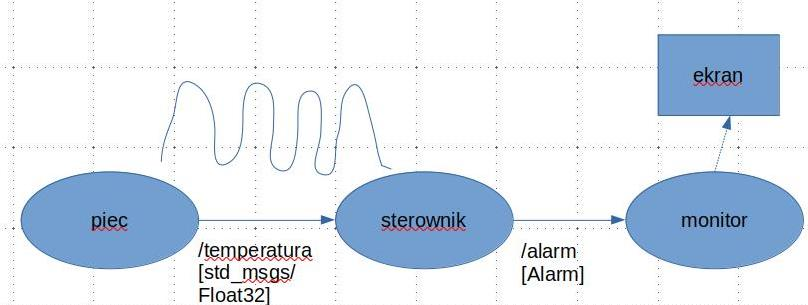
\includegraphics[width=1\linewidth]{focie/1.png}
    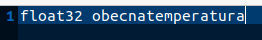
\includegraphics[width=1\linewidth]{focie/2.png}
    \caption{Wynik działania skryptu}
    \label{fig:1}
\end{figure}


Podsumowując, ten skrypt jest węzłem ROS, który publikuje wartości funkcji sinusoidalnej na temat 'y' z parametrami amplitudy i częstotliwości, które mogą być dynamicznie aktualizowane w trakcie działania węzła.


\begin{rozwiazanie}[: Regulator PID]
\end{rozwiazanie}

\begin{longlisting}
    \begin{minted}{python}
#!/usr/bin/python3

import rospy
from std_msgs.msg import Float32
import math

rospy.init_node('falka')
e = 0.0
y_mierz = 0.0
e_i = 0.0
e_d = 0.0
e_pop = 0.0
u = 0.0
pub = rospy.Publisher('y', Float32, queue_size=10)
rate = rospy.Rate(10.0)
t = 0

while not rospy.is_shutdown():
        dt = ros.get_param('dt')
        y_zad = rospy.get_param('y_zad')
        k_p = rospy.get_param('k_p')
        k_i = rospy.get_param('k_i')
        k_d = rospy.get_param('k_d')
        y_mierz = u
        e = y_zad - y_mierz
        e_i = e_i + (e * dt)
        e_d = (e - e_pop) / dt
        e_pop = e
        u = (k_p * e) + (k_i * e_i) + (k_d * e_d)
        msg = Float32()
        msg.data = u
        pub.publish(msg)
        rate.sleep()
        t += 1
    \end{minted}
\end{longlisting}

Oto kroki wykonywane przez ten skrypt:

\begin{enumerate}
    \item Importowanie niezbędnych bibliotek ROS oraz \verb|Float32| z \verb|std_msgs.msg| i \verb|math|.
    \item Inicjalizacja węzła ROS o nazwie ''falka'' za pomocą \verb|rospy.init_node('falka')|. Węzeł jest podstawową jednostką obliczeniową w ROS.
    \item Inicjalizacja zmiennych i publikatora (\verb|Publisher|) dla tematu ''y'' z typem \verb|Float32|.
    \item Ustawienie częstotliwości odświeżania na 10Hz za pomocą \verb|rate = rospy.Rate(10.0)|.
    \item Inicjalizacja zmiennej \verb|t| na 0, która służy do śledzenia czasu.
    \item Rozpoczęcie głównej pętli programu (\verb|while not rospy.is_shutdown()|).
    \item Pobranie parametrów \verb|dt|, \verb|y_zad|, \verb|k_p|, \verb|k_i|, \verb|k_d| za pomocą \verb|rospy.get_param()|. Parametry te są dostarczane przez zewnętrzne źródło, takie jak plik konfiguracyjny ROS.
    \item Uaktualnienie wartości zmiennej \verb|y_mierz| na podstawie wartości \verb|u|.
    \item Obliczenie błędu \verb|e| jako różnicy między wartością zadaną \verb|y_zad| a zmierzoną wartością \verb|y_mierz|.
    \item Obliczenie składnika całkującego błędu \verb|e_i| przez dodanie iloczynu błędu \verb|e| i czasu próbkowania \verb|dt| do wartości poprzedniej.
    \item Obliczenie składnika różniczkującego błędu \verb|e_d| jako iloraz różnicy błędu \verb|e| i poprzedniego błędu \verb|e_pop| przez czas próbkowania \verb|dt|.
    \item Zaktualizowanie wartości poprzedniego błędu \verb|e_pop| na bieżący błąd \verb|e|.
    \item Obliczenie wartości sterującej \verb|u| jako sumy iloczynów współczynników \verb|k_p|, \verb|k_i|, \verb|k_d| przez odpowiednie składniki błędów \verb|e|, \verb|e_i| i \verb|e_d|.
    \item Tworzenie obiektu wiadomości \verb|msg| typu \verb|Float32| i przypisanie mu wartości \verb|u|.
    \item Opublikowanie wiadomości na temat ''y'' za pomocą \verb|pub.publish(msg)|.
    \item Poczekanie na czas równy czasowi próbkowania \verb|dt| przy użyciu \verb|rate.sleep()|.
    \item Inkrementacja zmiennej \verb|t| o 1, aby śledzić upływ czasu.
\end{enumerate}


Ten skrypt jest ciągłą pętlą, która pobiera parametry zewnętrzne, oblicza sterowanie na podstawie regulatora PID i publikuje wartość sterowania na temat ''y'' w ROS.


\begin{figure}[H]
    \centering
    \includegraphics[width=0.6\linewidth]{focie/343277825_199878826279962_1738603146835426626_n.png}
    \includegraphics[width=1\linewidth]{focie/343327911_9343023112437947_4817743500631599258_n.png}
    \caption{Wynik działania skryptu}
    \label{fig:2}
\end{figure}

\subsection{Wnioski}
Zadanie zostało pomyślnie zakończone. Wykorzystanie parametrów w systemie ROS nie powoduje trudności podczas implementacji, ale wymaga biegłego modyfikowania kodu źródłowego. Zręczne edytowanie kodu programu umożliwia modyfikację parametrów w czasie rzeczywistym, jednak nie dotyczy to wszystkich. Stałe zadeklarowane jako kp, ki, kd można zmienić jedynie przez zatrzymanie głównego programu.

\end{document}
